\documentclass[a4paper,12pt]{BYUTextbook} 
\usepackage{amsmath}
\usepackage{makeidx}
\usepackage{graphicx}

\usepackage{tcolorbox}
\usepackage{breqn}

\title{\color{kj2}{\textsc{Physics Assignment}}}
\date{November 09, 2018}
\author{Karthik J}

\usepackage{xcolor}
\definecolor{kj1}{RGB}{113, 200, 55}
\definecolor{kj2}{RGB}{55,113,200}
\definecolor{kj3}{RGB}{141,95,211}

\usepackage{titlesec}


\titleformat{\section}
{\color{kj3}\normalfont\Large\bfseries}
{\color{kj3}\thesection}{1em}{}

\titleformat{\subsection}
{\color{kj1}\normalfont\large\bfseries}
{\color{kj1}\thesubsection}{1em}{}

\chead{Karthik J}
\rhead{}

\makeatletter
\renewcommand{\thesection}{%
	\ifnum\c@chapter<1 \@arabic\c@section
	\else \thechapter.\@arabic\c@section
	\fi
}
\makeatother

\begin{document}
	\maketitle
	\tableofcontents
		\newpage
		\chapter*{\vspace{-1.7in}Electromagnetic Waves}
		\section{Hertz Experiment}
			During the 1880s many scientists were trying to establish that light is an electromagnetic wave and the fact that such waves do exist. James Clerk Maxwell's mathematical theory of 1873 had predicted that electromagnetic disturbances should propagate through space at the speed of light and should exhibit the wave-like characteristics of light propagation.
			
			\marginfig{circuit}{The transmitter circuit \label{fig:transmitter}}
			
			\marginfig{receiver}{The loop of wire acting as a receiver \label{fig:receiver}}
			
			
			\marginfig{Hertz1}{Heinrich Hertz\label{fig:Hertz}}
			
			In 1887, Heinrich Hertz, a professor at Karlsruhe Polytechnic designed a set of experiments to test Maxwell's hypothesis.
			
			\subsection{Experiment set-up}
			\textbf{Transmitter.} Hertz used an oscillator made of polished brass knobs, each connected to an induction coil and separated by a tiny gap over which sparks could leap. The tiny gap acts as a capacitor (C), and the whole setup is equivalent to an LC-circuit. 
			\\
			\textbf{Receiver.} To detect the electromagnetic waves produced by the transmitter, Hertz made a simple receiver of a looped wire. At the ends of the loop were small knobs separated by a tiny gap. The receiver was placed several yards from the oscillator.
			
			\subsection{Working}
			This experiment is based on the fact that an oscillating electric charge radiates electromagnetic waves. The energy of these waves is due to the kinetic energy of the oscillating charge.
			
			Due to high voltage applied, the air in the small gap between the brass knobs gets ionised. This provides the path for the discharge of the plates. As a result, a spark begins to pass between the spheres. According to theory, if electromagnetic waves were spreading from the oscillator sparks, they would induce a current in the loop that would send sparks across the gap. 
			
			This did occur (as Hertz expected) when he turned on the oscillator., producing the first transmission of electromagnetic waves.
			
			The transmission of the electromagnetic waves was received by the loop of wire (which is the receiver), as indicated by the sparks produced across the brass knobs of the receiver.
			
			\subsection{Additional Observations}
			
			Hertz also noted the following observations about electromagnetic waves from his further experiments.
			
			\begin{itemize}
				\item Electrical conductors reflect the em waves. 
				\item The em waves can be focused by concave reflectors. 
				\item Insulators allow most of the waves to pass through.
			\end{itemize}
		
		\section{Electromagnetic Waves}
		
		\begin{tcolorbox}
			\subsection*{Maxwell's Equations}
			\begin{enumerate}
				\item Gauss' Law: \\$\nabla\cdot \vec{E} = \dfrac{\rho}{\varepsilon_0}$ 
				\item Gauss' Law of electromagnetism: \\$\nabla\cdot \vec{B} = 0 $
				\item Faraday's Law:\\
				$\nabla\times \vec{E} = - \dfrac{\partial \vec{B}}{\partial t} $
				\item Ampere-Maxwell Law:\\
				$\nabla\times \vec{B} = \mu_{0}\left(\vec{J} + \varepsilon_0 \dfrac{\partial \vec{E}}{\partial t}\right) $
			\end{enumerate}
		\end{tcolorbox}
		\marginfig[-1in]{Maxwell}{James Clerk Maxwell}
		For a given vector function F, the curl of the curl of F is given by
		\begin{equation}
			\nabla\times(\nabla\times \vec{F}) = \nabla(\nabla\cdot \vec{F}) - \nabla^{2}\vec{F}
		\end{equation}
		
		where, 
		
		$$ \nabla^{2} \vec{F} = \dfrac{\partial^{2} \vec{F}}{\partial x^{2}} + \dfrac{\partial^{2} \vec{F}}{\partial y^{2}} + \dfrac{\partial^{2} \vec{F}}{\partial z^{2}}$$
		
		(known as the \textit{Laplacian operator})
		
		Now, the third equation by Maxwell, known as \textit{Faraday's law}, is given by:
		
		\begin{equation}
			\nabla \times \vec{E} = - \dfrac{\partial \vec{B}}{\partial t}\outnote{Faraday's Law}
		\end{equation}
		
		Now, taking the curl of the above equation on both sides,
		
		$$ \nabla \times \left(\nabla \times \vec{E}\right) = \nabla \times \left(- \dfrac{\partial \vec{B}}{\partial t}\right) $$
		Using equation (1),
		$$\nabla \times \left(\nabla \times \vec{E}\right) = \nabla(\nabla\cdot \vec{E}) - \nabla^{2}\vec{E}\outnote{from equation (1)}$$
		$$\implies \nabla(\nabla\cdot \vec{E}) - \nabla^{2}\vec{E} = \nabla \times \left(- \dfrac{\partial \vec{B}}{\partial t}\right)$$
		Because the curl is simply a group of spatial derivatives, it can be brought
		inside the derivative with respect to time on the right side of the equation:
		$$\implies \nabla(\nabla\cdot \vec{E}) - \nabla^{2}\vec{E} = \left(- \dfrac{\partial (\nabla \times \vec{B})}{\partial t}\right)$$
		Now, substituting the expression for $\nabla\times B$ from Maxwell's fourth equation,
		$$\implies \nabla(\nabla\cdot \vec{E}) - \nabla^{2}\vec{E} =  \left(- \dfrac{\partial \left( \mu_{0}\left(\vec{J} + \varepsilon_0 \dfrac{\partial \vec{E}}{\partial t}\right) \right)}{\partial t}\right) \outnote{from Ampere-Maxwell equation}$$
		From Maxwell's first equation, substituting the value of $\nabla\cdot E$,
		$$\nabla\left(\dfrac{\rho}{\varepsilon_0}\right) - \nabla^{2}\vec{E} = \left(- \dfrac{\partial \left( \mu_{0}\left(\vec{J} + \varepsilon_0 \dfrac{\partial \vec{E}}{\partial t}\right) \right)}{\partial t}\right) \outnote{from Gauss law}$$
		$$\implies \nabla\left(\dfrac{\rho}{\varepsilon_0}\right) - \nabla^{2}\vec{E} = -\dfrac{\partial\left(\mu_{0}\vec{J}\right)}{\partial t} - \mu_{0}\varepsilon_{0}\dfrac{\partial^{2}\vec{E}}{\partial t^{2}} $$
		In the absence of charge, $\rho = 0$,  and in the absence of current $\vec{J} = 0$. Under these conditions, the first terms on both sides are zero, and the negative signs on the remaining terms cancel. What remains is:
		
		\begin{equation}
			\nabla^{2}\vec{E} = \mu_{0}\varepsilon_{0} \dfrac{\partial \vec{E}}{\partial t^{2}} \outnote{Electromagnetic wave equation}
		\end{equation}
		
		This is a second-order differential equation that relates an electric field that varies in space and time. That is, it describes a wave, and this differential equation is known in physics as the \textit{wave equation}. The general form of the wave equation (for any wave) is
		
		$$ \nabla^2 \vec{F} = \dfrac{1}{v^2} \dfrac{\partial^2 \vec{F}}{\partial t^2} \outnote{Wave Equation}$$
		
		where $v$ is the velocity of the wave. The function $\vec{F}$ can be expressed in terms of sine and cosine functions or as an imaginary exponential function; the exact expression for an $\vec{E}$ wave (light) depends on the boundary conditions and the initial value at some point in space.
		
		This wave equation implies that
		
		\begin{equation}
			v_{\text{light}} = \dfrac{1}{\sqrt{\mu_{0}\varepsilon_{0}}} \outnote{Velocity of electromagnetic wave}
		\end{equation}
		
		Hence  Maxwell concluded that light is a wave of an electric field that had a velocity of $\left(\dfrac{1}{\sqrt{\mu_{0}\varepsilon_{0}}}\right)$.
				
		If we take the curl of the Ampère–Maxwell law and perform similar substitutions, we get 
		
		$$ \nabla^2 \vec{B} = \mu_{0}\varepsilon_{0}\dfrac{\partial \vec{B}}{\partial t^2} $$
		
		This is the same form of the wave equation, so we have the same conclusions: light is a wave of a magnetic field having a velocity of $\left(\dfrac{1}{\sqrt{\mu_{0}\varepsilon_{0}}}\right)$.
		
		However, because of Faraday’s law (Maxwell’s third equation), the electric field and the magnetic field associated with a light wave are perpendicular to each other.
		
		\begin{figure}[!htb]
			\inneralign{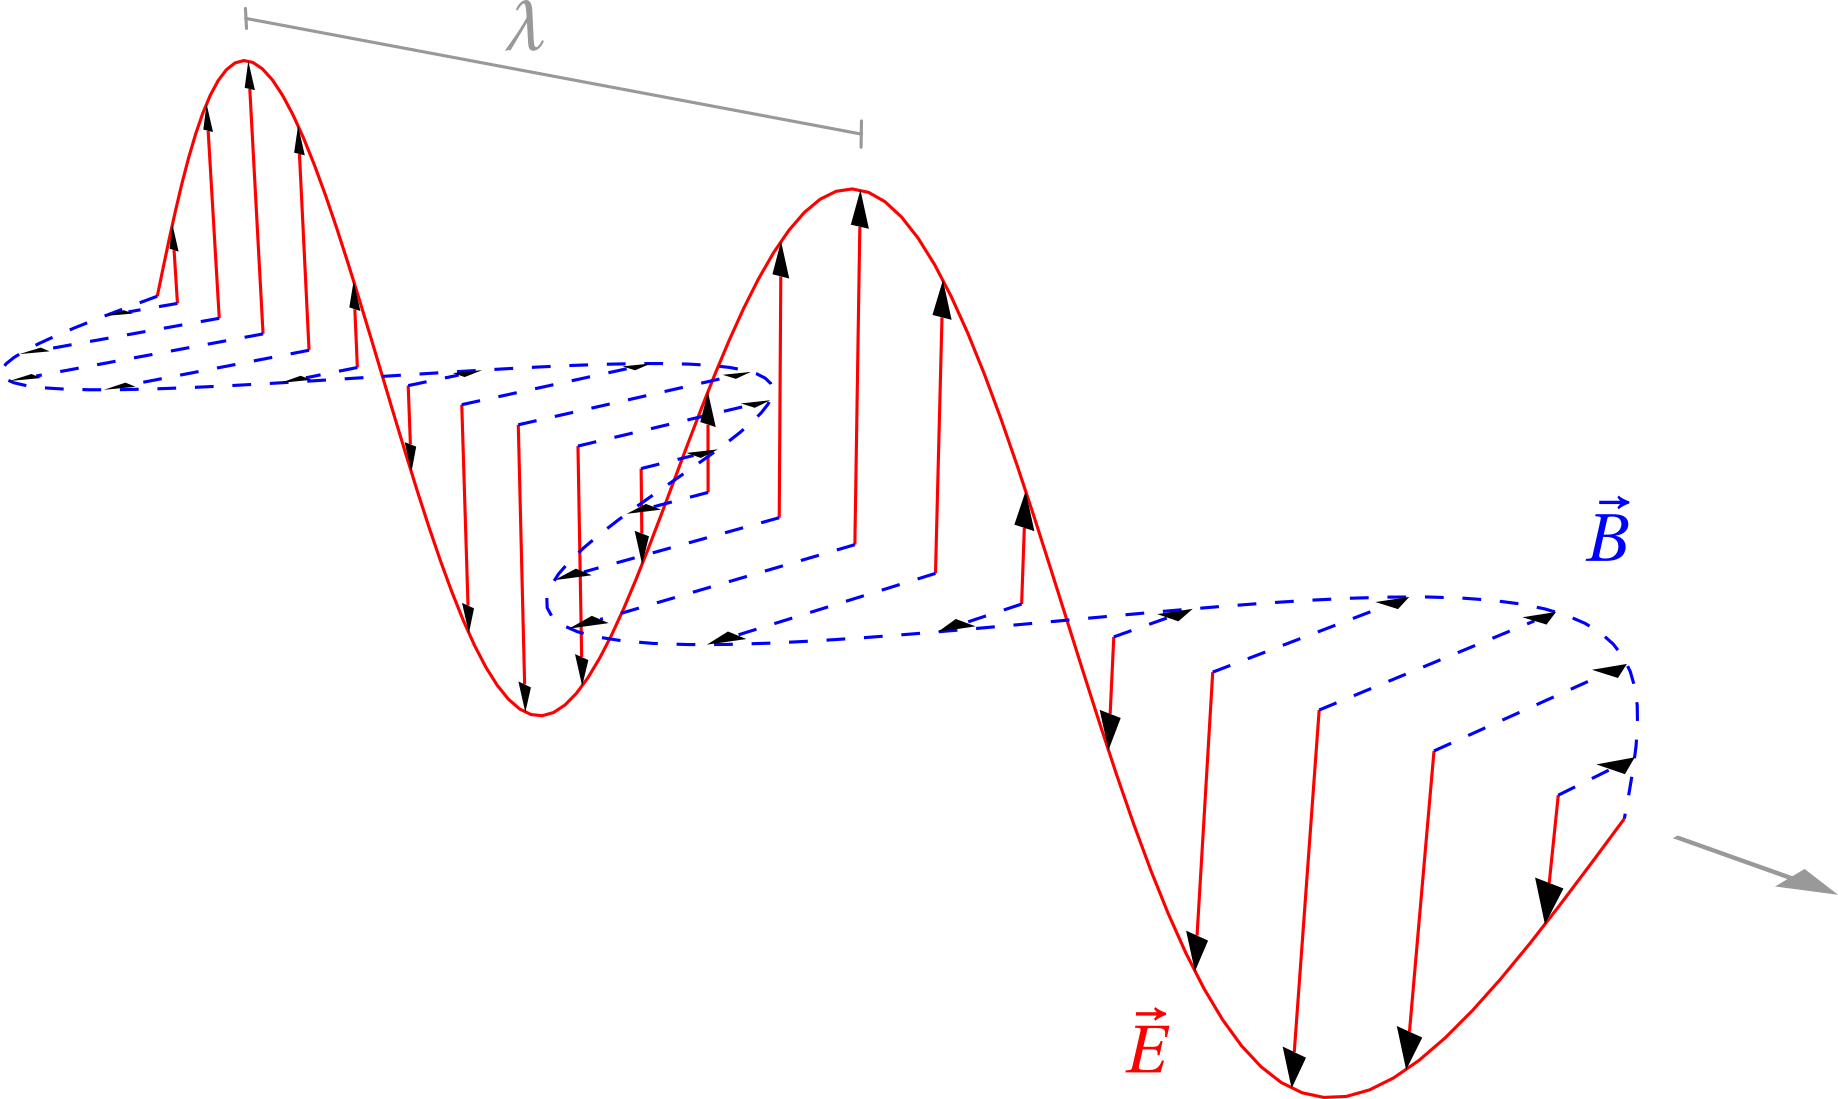
\includegraphics{em.png}}
			\caption{\label{fig:8.6} Propagation of electromagnetic waves
			}
		\end{figure} 
		
\end{document}